%package list
\documentclass{article}
\usepackage[top=3cm, bottom=3cm, outer=3cm, inner=3cm]{geometry}
\usepackage{graphicx}
\usepackage{url}
%\usepackage{cite}
\usepackage{hyperref}
\usepackage{array}
%\usepackage{multicol}
\newcolumntype{x}[1]{>{\centering\arraybackslash\hspace{0pt}}p{#1}}
\usepackage{natbib}
\usepackage{pdfpages}
\usepackage{multirow}
\usepackage{multirow}
\usepackage[normalem]{ulem}
\useunder{\uline}{\ul}{}
\usepackage{amsmath}
\usepackage{float}
\usepackage{multicol}
\usepackage{subcaption}


% para tener url cortas en bib
\let\oldUrl\url
\renewcommand{\url}[1]{\href{#1}{Enlace}}
%

%%%%%%%%%%%%%%%%%%%%%%%%%%%%%%%%%%%%%%%%%%%%%%%%%%%%%%%%%%%%%%%%%%%%%%%%%%%%
%%%%%%%%%%%%%%%%%%%%%%%%%%%%%%%%%%%%%%%%%%%%%%%%%%%%%%%%%%%%%%%%%%%%%%%%%%%%
\newcommand{\csemail}{vmachacaa@ulasalle.edu.pe}
%\newcommand{\csdocente}{MSc. Vicente Enrique Machaca Arceda}
\newcommand{\csdocente}{Vicente Machaca Arceda \\ Enzo Velásquez Lobatón \\
	Carlo Corrales Delgado\\
	Oscar Ramirez Valdez
	}
\newcommand{\cscurso}{Computación de Alto Desempeño}
\newcommand{\csuniversidad}{Universidad Nacional de San Agustín de Arequipa}
\newcommand{\csescuela}{Doctorado en Ciencias de la Computación}
\newcommand{\cspracnr}{04}
\newcommand{\cstema}{Spark}
%%%%%%%%%%%%%%%%%%%%%%%%%%%%%%%%%%%%%%%%%%%%%%%%%%%%%%%%%%%%%%%%%%%%%%%%%%%%
%%%%%%%%%%%%%%%%%%%%%%%%%%%%%%%%%%%%%%%%%%%%%%%%%%%%%%%%%%%%%%%%%%%%%%%%%%%%


\usepackage[english,spanish]{babel}
\usepackage[utf8]{inputenc}
\AtBeginDocument{\selectlanguage{spanish}}
\renewcommand{\figurename}{Figura}
\renewcommand{\refname}{Referencias}
\renewcommand{\tablename}{Tabla} %esto no funciona cuando se usa babel
\AtBeginDocument{%
	\renewcommand\tablename{Tabla}
}

\usepackage{fancyhdr}
\pagestyle{fancy}
\fancyhf{}
\setlength{\headheight}{30pt}
\renewcommand{\headrulewidth}{1pt}
\renewcommand{\footrulewidth}{1pt}
\fancyhead[L]{\raisebox{-0.2\height}{
\includegraphics[width=3cm]{img/logo_unsa}}}
\fancyhead[C]{}
\fancyhead[R]{\fontsize{7}{7}\selectfont	\csuniversidad \\ \csescuela \\ \textbf{\cscurso} }
\fancyfoot[L]{Vicente, Enzo, Oscar y Carlo}
\fancyfoot[C]{\cscurso}
\fancyfoot[R]{Página \thepage}


% para el codigo fuente
\usepackage{listings}
\usepackage{color}
\definecolor{dkgreen}{rgb}{0,0.6,0}
\definecolor{gray}{rgb}{0.5,0.5,0.5}
\definecolor{mauve}{rgb}{0.58,0,0.82}
\lstset{frame=tb,
	language=Python,
	aboveskip=3mm,
	belowskip=3mm,
	showstringspaces=false,
	columns=flexible,
	basicstyle={\small\ttfamily},
	numbers=none,
	numberstyle=\tiny\color{gray},
	keywordstyle=\color{blue},
	commentstyle=\color{dkgreen},
	stringstyle=\color{mauve},
	breaklines=true,
	breakatwhitespace=true,
	tabsize=3
}



\begin{document}
	
	
	
	
\begin{titlepage}
	
	\newcommand{\HRule}{\rule{\linewidth}{0.5mm}} % Defines a new command for the horizontal lines, change thickness here
	
	\center % Center everything on the page
	
	%----------------------------------------------------------------------------------------
	%	HEADING SECTIONS
	%----------------------------------------------------------------------------------------
	
	\textsc{\LARGE \csuniversidad}\\[1.5cm] % Name of your university/college
	\textsc{\Large \cscurso}\\[0.5cm] % Major heading such as course name
	%\textsc{\large Assignment 1}\\[0.5cm] % Minor heading such as course title
	
	%----------------------------------------------------------------------------------------
	%	TITLE SECTION
	%----------------------------------------------------------------------------------------
	
	\vspace{2cm}
	
	\HRule \\[0.4cm]
	{ \huge \bfseries \cstema}\\[0.4cm] % Title of your document
	\HRule \\[1.5cm]
	
	%----------------------------------------------------------------------------------------
	%	AUTHOR SECTION
	%----------------------------------------------------------------------------------------
	
	\begin{minipage}{0.4\textwidth}
		\begin{flushleft} \large
			\emph{Alumnos:}\\
			\csdocente
		\end{flushleft}
	\end{minipage}
	~
	\begin{minipage}{0.4\textwidth}
		\begin{flushright} \large
			\emph{Docente:} \\
			PhD. Alvaro Mamani Aliaga
		\end{flushright}
	\end{minipage}\\[2cm]
	
	% If you don't want a supervisor, uncomment the two lines below and remove the section above
	%\Large \emph{Author:}\\
	%John \textsc{Smith}\\[3cm] % Your name
	
	%----------------------------------------------------------------------------------------
	%	DATE SECTION
	%----------------------------------------------------------------------------------------
	
	{\large \today}\\[2cm] % Date, change the \today to a set date if you want to be precise
	
	%----------------------------------------------------------------------------------------
	%	LOGO SECTION
	%----------------------------------------------------------------------------------------
	
	
\includegraphics[width=100px, keepaspectratio]{img/unsa}\\[1cm] % Include a department/university logo - this will require the graphicx package
	
	%----------------------------------------------------------------------------------------
	
	\vfill % Fill the rest of the page with whitespace
	
\end{titlepage}	
	
	
	

	
	
\tableofcontents
\newpage	
	

	
		
	
\section{Introducción}

La principal función del motor de Spark, \cite{apacheSpark} es planificar, asignar y monitorizar aplicaciones multitarea para el procesamiento de datos sobre las máquinas del clúster que serán las encargadas de ejecutar las tareas. 

Apache Spark, \cite{ApacheBigData}, \cite{spark2018apache}, \cite{spark2010spark} es un sistema de computación distribuido de código abierto basado en Hadoop, pensado para el análisis y procesamiento de datos en los campos del Big Data y el Machine Learning. Se trata del mayor proyecto de código abierto en el campo del análisis y procesamiento de datos. 

Clasificación, una tarea habitual en el aprendizaje automático, es el proceso de ordenación de datos de entrada en categorías. Es trabajo de un algoritmo de clasificación averiguar cómo asignar "etiquetas" a los datos de entrada que usted proporciona. Por ejemplo, podría pensar en un algoritmo de aprendizaje automático que acepte información bursátil como entrada. 

La regresión logística es el algoritmo que se usa para la clasificación. La API de regresión logística de Spark es útil para la clasificación binaria, o para la clasificación de datos de entrada en uno de los dos grupos. 

En resumen, el proceso de regresión logística produce una función logística. se utiliza la función para predecir la probabilidad de que un vector de entrada pertenezca a un grupo u otro grupo.

\section{Aplicaciones}

Primero se implementó el algoritmo para predecir si un pasajero sobrevivió o no al naufragio del Titanic, para lo cual se realizaron las siguientes actividades, primero se revisó el conjunto de datos del Titanic y luego se trató de predecir si una persona sobrevivió al naufragio. El objetivo es predecir si un pasajero sobrevivió o no. Para ello se toman un valor binario (0,1) que significa: 0 por no sobrevivir, 1 por sobrevivir.

Y luego, se implementó el algoritmo de páginas de compras, que consiste en predecir si un visitante de la página realizará una compra o solo está de visita de acuerdo con las acciones que realiza dentro de la página. El objetivo es identificar a los visitantes que compran dentro de la página web.


\section{Implementación}

Para la implementación se planteo la solución de dos problemas:
\begin{itemize}
    \item ¿Como saber si un pasajero del Titanic podría sobrevivir?
    \item ¿Como saber si un visitante se volveria cliente a partir de información recolectada de sus acciones en la página de compras?
\end{itemize}

\subsection{Titanic}

La base de datos del Titanic, \cite{datapicker} contiene 891 muestras y 11 atributos. Esta base datos ha recolectado información de los pasajeros al Titanic, como por ejemplo, edad, sexo, con hijos, etc. Y en base a esa información un modelo debería poder clasificar si un pasajero sobrevive o no al hundimiento del Titanic. Los atributos son:

\begin{lstlisting}
 |-- PassengerId: integer (nullable = true)
 |-- Survived: integer (nullable = true)
 |-- Pclass: integer (nullable = true)
 |-- Name: string (nullable = true)
 |-- Sex: string (nullable = true)
 |-- Age: double (nullable = true)
 |-- SibSp: integer (nullable = true)
 |-- Parch: integer (nullable = true)
 |-- Ticket: string (nullable = true)
 |-- Fare: double (nullable = true)
 |-- Cabin: string (nullable = true)
 |-- Embarked: string (nullable = true)
\end{lstlisting}

Para solucionar este problema, se utilizo Regresión Logistíca. Este es el código fuente:

\begin{lstlisting}
from pyspark.sql import SparkSession
from pyspark.ml.classification import LogisticRegression

spark = SparkSession.builder.appName('titanic_logreg').getOrCreate()
df = spark.read.csv('titanic.csv', inferSchema = True, header = True)
df.show(3)
df.printSchema()


my_col = df.select(['Survived','Pclass','Sex','Age','SibSp','Parch','Fare','Embarked'])
final_data = my_col.na.drop()

from pyspark.ml.feature import (VectorAssembler, StringIndexer, VectorIndexer, OneHotEncoder)

gender_indexer = StringIndexer(inputCol = 'Sex', outputCol = 'SexIndex')
gender_encoder = OneHotEncoder(inputCol='SexIndex', outputCol = 'SexVec')
embark_indexer = StringIndexer(inputCol = 'Embarked', outputCol = 'EmbarkIndex')
embark_encoder = OneHotEncoder(inputCol = 'EmbarkIndex', outputCol = 'EmbarkVec')

assembler = VectorAssembler(inputCols = ['Pclass', 'SexVec', 'Age', 'SibSp', 'Parch', 'Fare', 'EmbarkVec'], outputCol = 'features')


from pyspark.ml import Pipeline

log_reg = LogisticRegression(featuresCol = 'features', labelCol = 'Survived')

pipeline = Pipeline(stages = [gender_indexer, embark_indexer, 
                             gender_encoder, embark_encoder,
                             assembler, log_reg])

train, test = final_data.randomSplit([0.7, 0.3])
fit_model = pipeline.fit(train)
results = fit_model.transform(test)
results.select('prediction', 'Survived').show(3)

from pyspark.ml.evaluation import BinaryClassificationEvaluator

eval = BinaryClassificationEvaluator(rawPredictionCol = 'rawPrediction', labelCol = 'Survived')
AUC = eval.evaluate(results)
print("\n\nAUC", AUC, '\n\n')


\end{lstlisting}

\subsection{Página de compras}

La base de datos del Compras, contiene 73487 muestras y 16 atributos. Esta base de datos contiene información recolectada de una página de compras con acciones de los usuarios. El problema consiste en saber si un visitante a la página se puede volver comprador en base a las acciones realizadas en la página. Los atributos son:

\begin{lstlisting}
 |-- Visit_Number_Bucket: string (nullable = true)
 |-- Page_Views_Normalized: double (nullable = true)
 |-- label: integer (nullable = true)
 |-- Internal_Search_Successful_Normalized: double (nullable = true)
 |-- Internal_Search_Null_Normalized: double (nullable = true)
 |-- Email_Signup_Normalized: double (nullable = true)
 |-- Total_Seconds_Spent_Normalized: double (nullable = true)
 |-- Store_Locator_Search_Normalized: double (nullable = true)
 |-- Mapped_Last_Touch_Channel: string (nullable = true)
 |-- Mapped_Mobile_Device_Type: string (nullable = true)
 |-- Mapped_Browser_Type: string (nullable = true)
 |-- Mapped_Entry_Pages: string (nullable = true)
 |-- Mapped_Site_Section: string (nullable = true)
 |-- Mapped_Promo_Code: string (nullable = true)
 |-- Maped_Product_Name: string (nullable = true)
 |-- Mapped_Search_Term: string (nullable = true)
 |-- Mapped_Product_Collection: string (nullable = true)
\end{lstlisting}

Para solucionar este problema, se utilizo una Red Neuronal artificial. Este es el código fuente:

\begin{lstlisting}

from pyspark.sql import SparkSession
spark = SparkSession.builder.appName('deep_learning').getOrCreate()
import os
import numpy as np
import pandas as pd
from pyspark.sql.types import *

data = spark.read.csv('dl_data.csv', header=True, inferSchema=True)
data.printSchema()


data = data.withColumnRenamed('Orders_Normalized', 'label')
data.printSchema()

from pyspark.ml.feature import OneHotEncoder, VectorAssembler, StringIndexer
from pyspark.ml import Pipeline
from pyspark.sql.functions import udf, StringType
from pyspark.ml.evaluation import MulticlassClassificationEvaluator
from pyspark.ml.classification import MultilayerPerceptronClassifier

train, validation, test = data.randomSplit([0.7, 0.2, 0.1], 1234)

categorical_columns = [item[0] for item in data.dtypes if item[1].startswith(
    'string')]
numeric_columns = [item[0] for item in data.dtypes if item[1].startswith(
    'double')]
indexers = [StringIndexer(inputCol=column, outputCol='{0}_index'.format(
    column)) for column in categorical_columns]

featuresCreator = VectorAssembler(
    inputCols=[indexer.getOutputCol() for indexer in indexers] + numeric_columns,
    outputCol='features')
layers = [len(featuresCreator.getInputCols()), 4, 2, 2]

classifier = MultilayerPerceptronClassifier(labelCol='label',
                                            featuresCol='features',
                                            maxIter=100,
                                            layers=layers,
                                            blockSize=128,
                                            seed=1234)

pipeline = Pipeline(stages=indexers + [featuresCreator, classifier])
model = pipeline.fit(train)


train_output_df = model.transform(train)
validation_output_df = model.transform(validation)
test_output_df = model.transform(test)


train_predictionAndLabels = train_output_df.select('prediction', 'label')
validation_predictionAndLabels = validation_output_df.select('prediction', 'label')
test_predictionAndLabels = test_output_df.select('prediction', 'label')

metrics = ['weightedPrecision', 'weightedRecall', 'accuracy']
for metric in metrics:
  evaluator = MulticlassClassificationEvaluator(metricName=metric)
  print('Train ' + metric + ' = ' + str(evaluator.evaluate(
      train_predictionAndLabels)))
  print('Validation ' + metric + ' = ' + str(evaluator.evaluate(
      validation_predictionAndLabels)))
  print('Test ' + metric + ' = ' + str(evaluator.evaluate(
      test_predictionAndLabels)))
\end{lstlisting}

%%%%%%%%%%%%%%%%%%%%%%%%%%%%%%%%%%%%%%%%%%%%%%%%%%%%%%%%%%%%%%%%%
%%%%%%%%%%%%%%%%%%%%%%%%%%%%%%%%%%%%%%%%%%%%%%%%%%%%%%%%%%%%%%%%%
%%%%%%%%%%%%%%%%%%%%%%%%%%%%%%%%%%%%%%%%%%%%%%%%%%%%%%%%%%%%%%%%%
%%%%%%%%%%%%%%%%%%%%%%%%%%%%%%%%%%%%%%%%%%%%%%%%%%%%%%%%%%%%%%%%%

\section{Resultados}

Cada ejemplo ha sido evaluado en \textit{Spark}, con el comando: \textit{spark-submit  --master local[4]  script.py}. En la Figura \ref{fig:spark_1} y \ref{fig:spark_2}, se muestra el resultado luego de entrenar el modelo de regresión logística con la base de datos de Titanic. Como podemos ver, se logro un AUC de 0.84.

\begin{figure}[H]
    \centering
    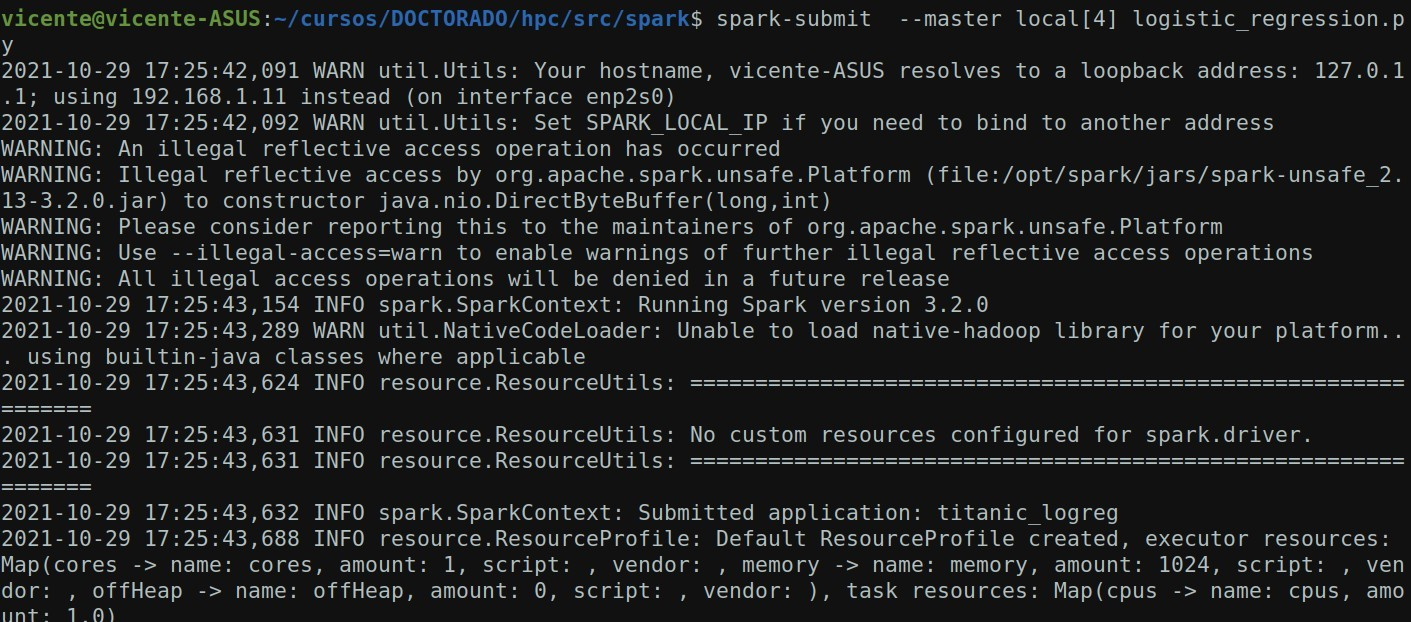
\includegraphics[width=15cm]{tareas/img/spark_1.jpg}
    \caption{Ejecución del modelo de Regresión logística.}
    \label{fig:spark_1}
\end{figure}

\begin{figure}[H]
    \centering
    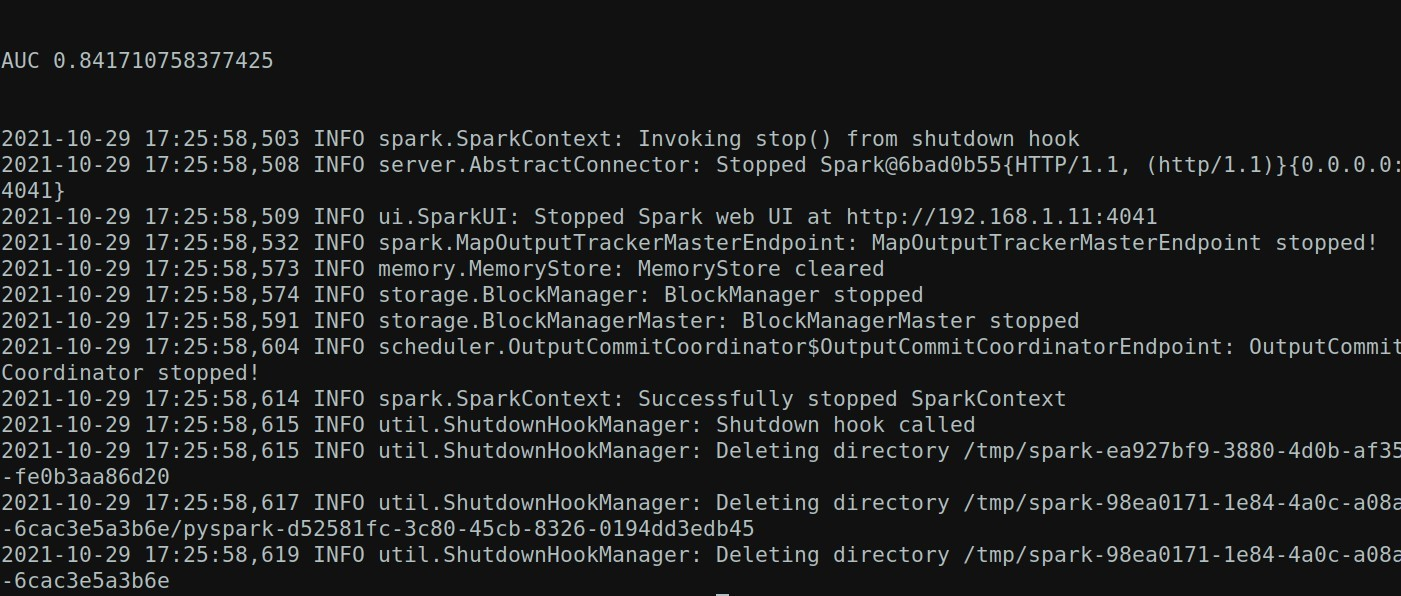
\includegraphics[width=15cm]{tareas/img/spark_2.jpg}
    \caption{Ejecución del modelo de Regresión logística.}
    \label{fig:spark_2}
\end{figure}

En la Figura \ref{fig:spark_3} y \ref{fig:spark_3}, se muestra el resultado luego de entrenar el modelo de redes neuronales con la base de datos de Compras por internet. En este caso obtuvimos un acierto de 0.98.


\begin{figure}[H]
    \centering
    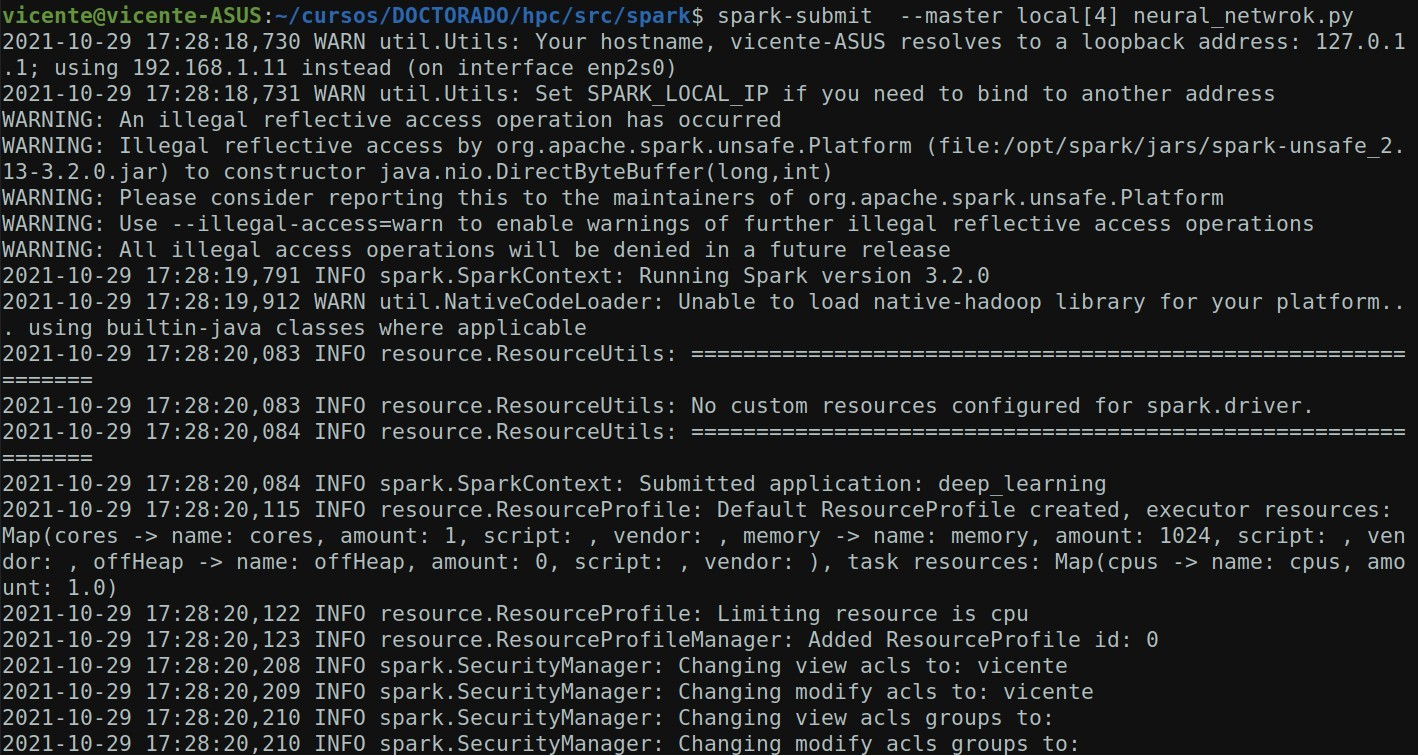
\includegraphics[width=15cm]{tareas/img/spark_3.jpg}
    \caption{Ejecución de la red neuronal.}
    \label{fig:spark_3}
\end{figure}

\begin{figure}[H]
    \centering
    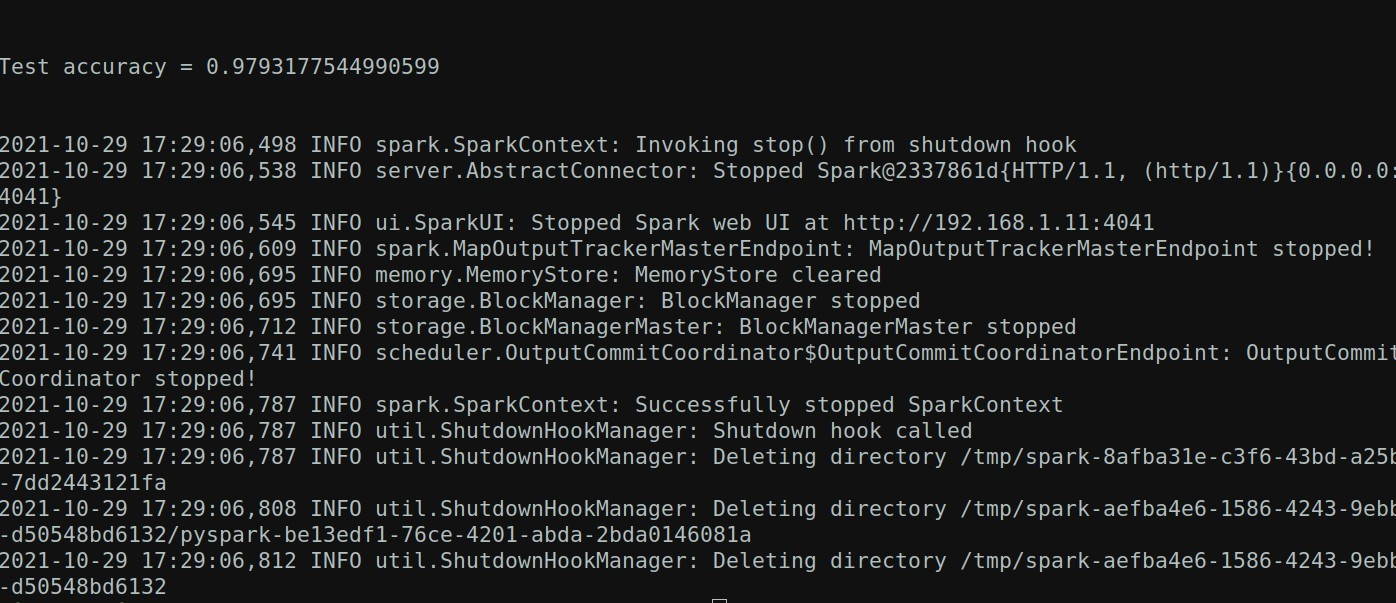
\includegraphics[width=15cm]{tareas/img/spark_4.jpg}
    \caption{Ejecución de la red neuronal.}
    \label{fig:spark_4}
\end{figure}


\section{Conclusiones}

\begin{itemize}
    \item Spark permite planificar, asignar y monitorizar aplicaciones multitarea para el procesamiento de datos sobre clústers.  Es una aplicación distribuida de código abierto basado en Hadoop para el análisis y procesamiento de datos en Big Data y Machine Learning.
    \item Los algoritmos implementados en este proyecto permiten realizar costosas operaciones en un tiempo reducido. 
    \item En el ejemplo, la base de datos ha recolectado información de los pasajeros al Titanic, como por ejemplo, edad, sexo, con hijos, etc. Y en base a esa información un modelo debería poder clasificar si un pasajero sobrevive o no al hundimiento del crucero. 
\end{itemize}
 


\bibliographystyle{apalike}
%\bibliographystyle{IEEEtranN}
\bibliography{bibliography}

\end{document}